\subsection{Biological testing\label{sec:bio1}}

\subsubsection{Autoinducer-antibiotic conjugates}

The eight triazoles made in \ref{sec:Tris} (see \ref{fgr:finals_1}) were tested for antibacterial and anti-biofilm activity in \textit{P. aeruginosa} PAO1\cite{Stover2000} and YM64\cite{Morita2001}.
PAO1 is the \textit{P. aeruginosa} wild-type strain.
YM64 is a mutant lacking all of the four major \textit{mex} operons for multidrug efflux pumps: \textit{mexAB-oprM}, \textit{mexXY}, \textit{mexCD-oprJ} and \textit{mexEF-oprN}, making it more sensitive to many antibiotics and hence able to show up moderate effects more clearly.

\begin{figure}[H]
	\begin{center}
		\schemeref[HL2T4Cip]{cmpd:HL2T4Cip}
		\schemeref[HL4T4Cip]{cmpd:HL4T4Cip}
		\schemeref[HL6T4Cip]{cmpd:HL6T4Cip}
		\schemeref[6HHQT4Cip]{cmpd:6HHQT4Cip}
		\schemeref[HL4T4Tri]{cmpd:HL4T4Tri}
		\schemeref[HL6T4Tri]{cmpd:HL6T4Tri}
		\schemeref[6HHQT4Tri]{cmpd:6HHQT4Tri}
		\schemeref[PQST4Tri]{cmpd:PQST4Tri}	
		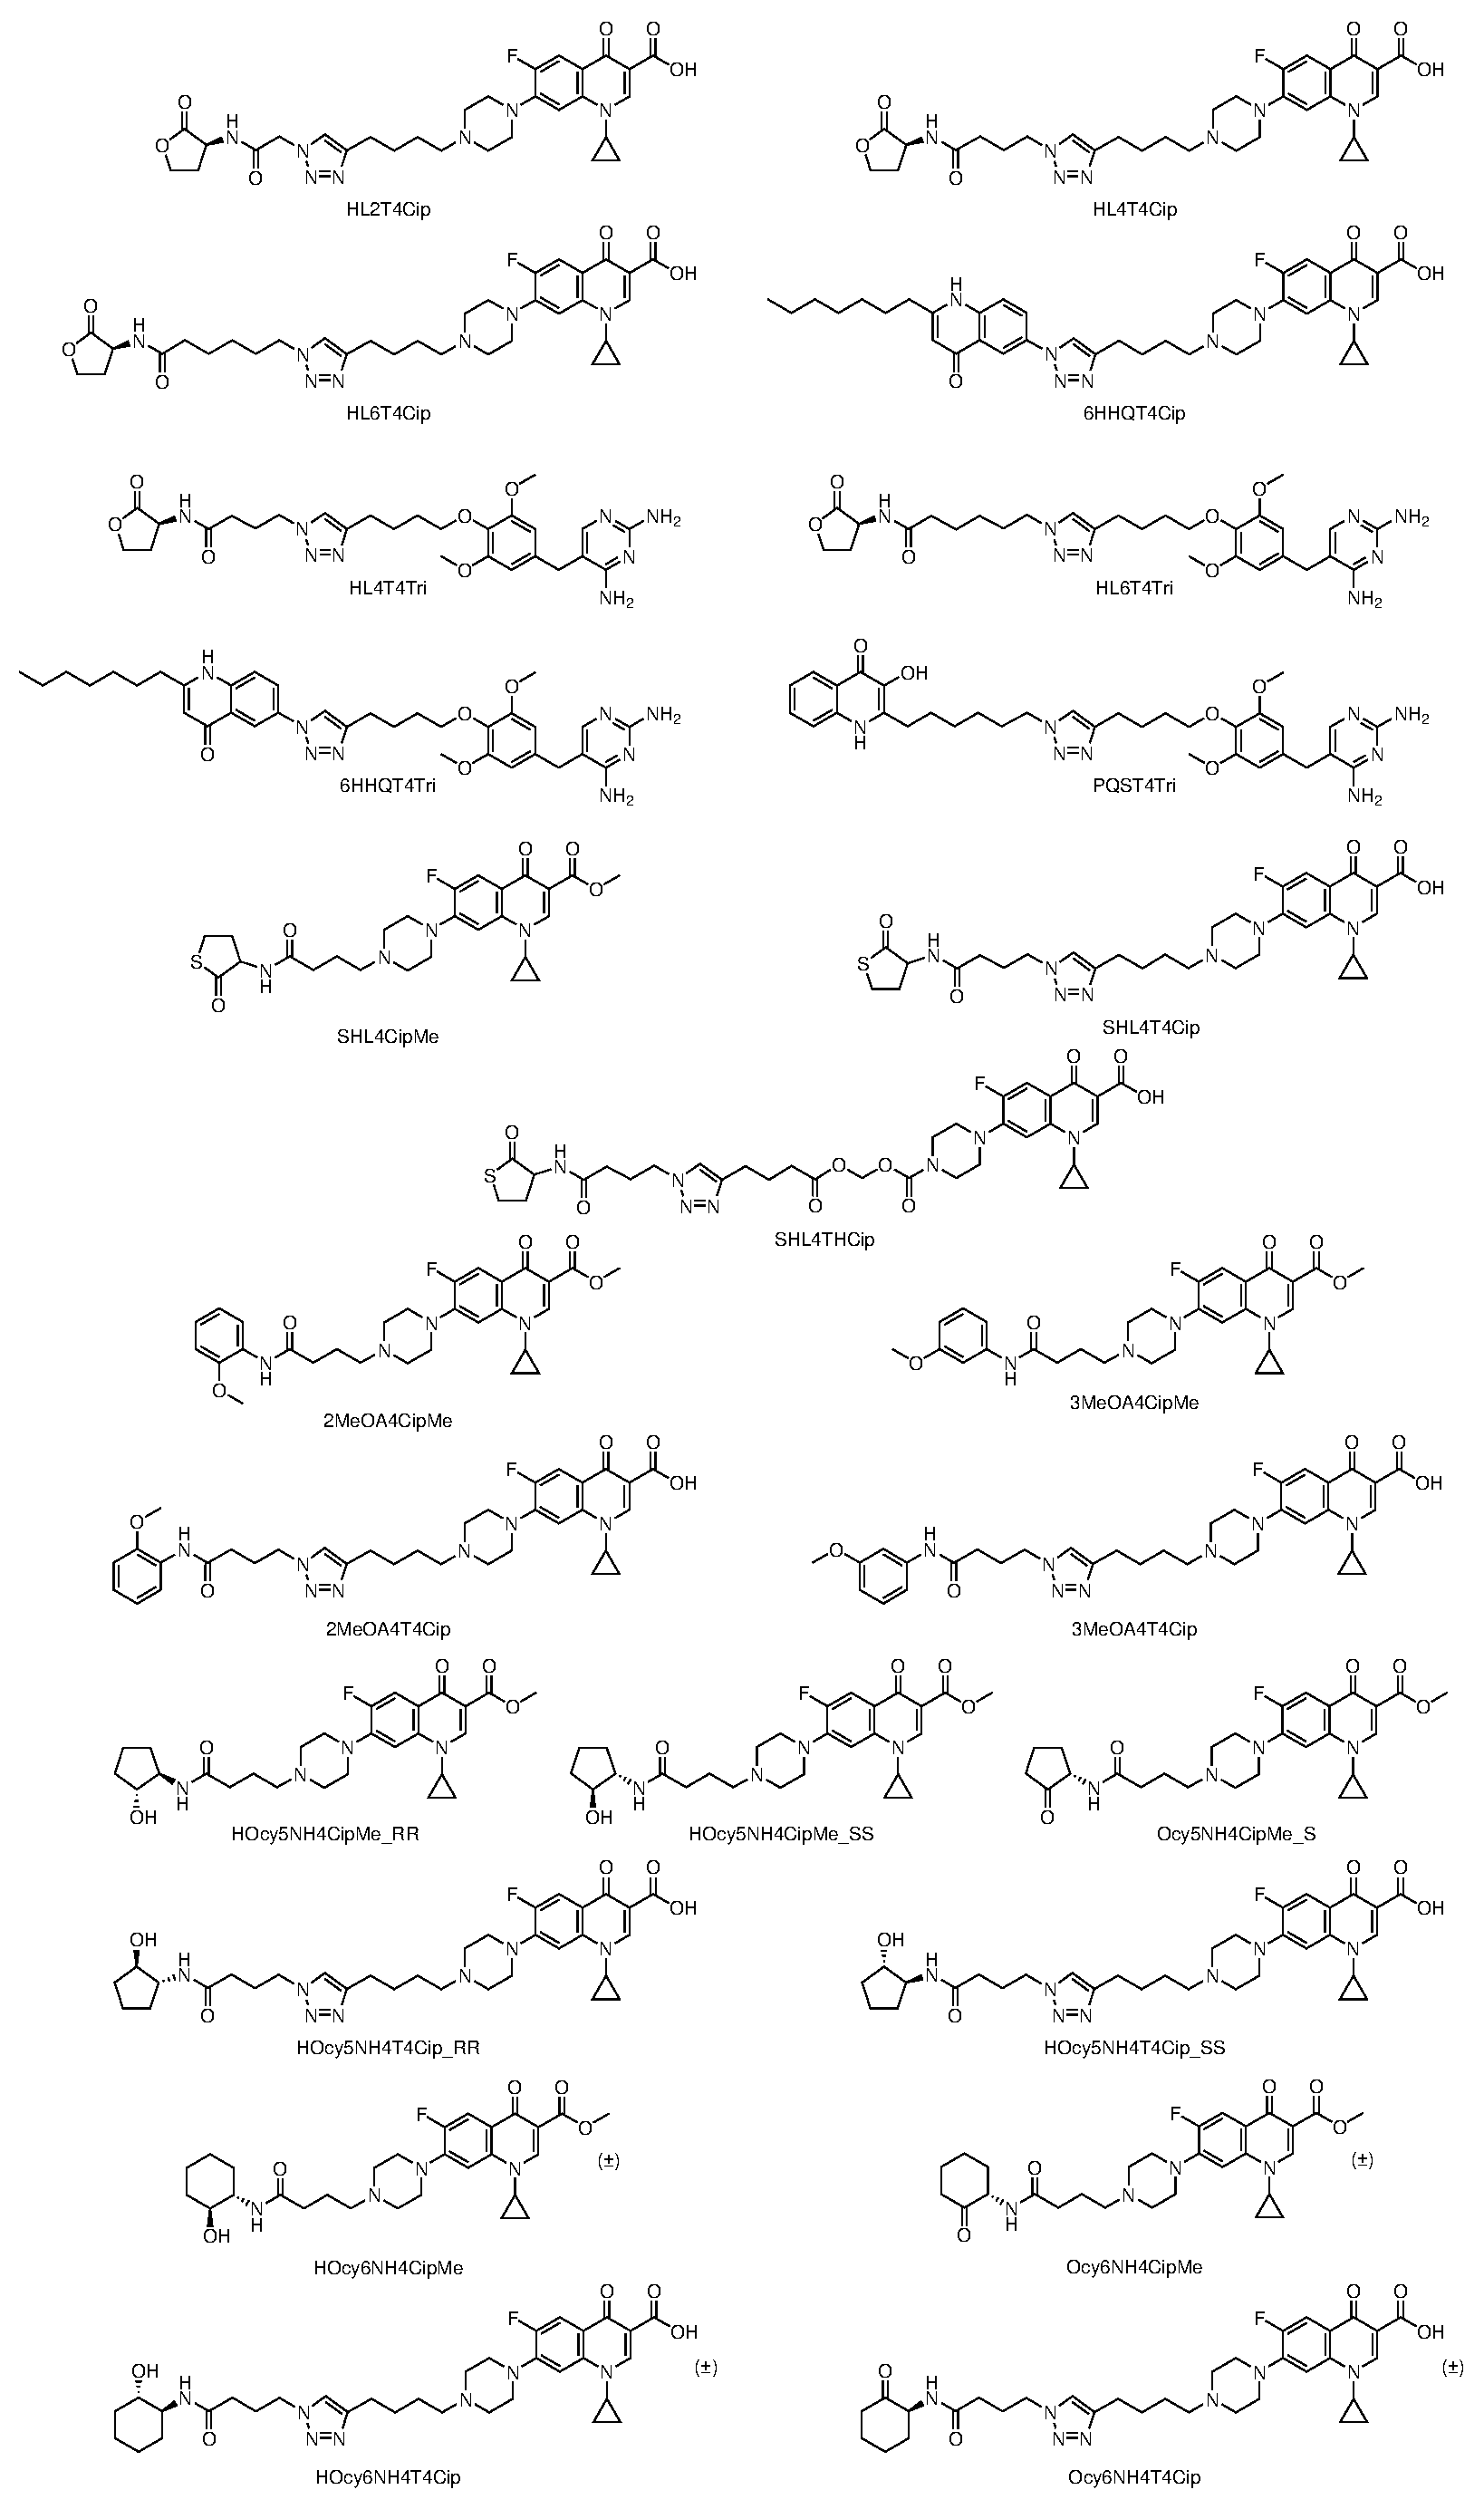
\includegraphics[width=\textwidth]{finals_1}
		\caption{The autoinducer-antibiotic conjugates.
 		\label{fgr:finals_1}}
	\end{center}
\end{figure}

\subsubsubsection{Antibacterial and anti-biofilm testing against YM64}

In YM64 at 5 h the HSL-Cip conjugates \compound{cmpd:HL2T4Cip}, \compound{cmpd:HL4T4Cip} and \compound{cmpd:HL6T4Cip} showed slight activity at the highest concentration, but not as much as ciprofloxacin \compound{cmpd:Cip}.
This activity was not visible by 24 h (see \ref{fgr:YM64_24h}) and the compounds had no effect on biofilm formation (see \ref{fgr:YM64_biofilms}).

A dose-dependant response was expected for these results, however this was not seen except for a slight effect at 5 h in YM64 for some compounds. The dose-dependant response might potentially be seen if higher concentrations were tested, although there could be problems with compound solubility. Conversely, the dose-dependant response might be seen for ciprofloxacin \compound{cmpd:Cip} if lower concentrations were tested. Smaller `steps' in concentration could also be tested after establishing the range over which the dose-dependant response is seen.

The very high readings in the biofilm assays for ciprofloxacin \compound{cmpd:Cip} (see \ref{fgr:YM64_biofilms} and \ref{fgr:PAO1_biofilms}) could be due to sub-MIC concentrations of the antibiotic causing the bacteria to respond by forming a protective biofilm. This effect has been reported with cefotaxim, amoxicillin, azithromycin\cite{Aka2015,Hoffman2005}, tobramycin, amikacin, streptomycin and gentamicin, but oddly not with ciprofloxacin \compound{cmpd:Cip}\cite{Gupta2016,Machado2013}, although this could be due to the exact conditions of growth.

\begin{figure}[H]
	\begin{center}
		\includegraphics[width=0.9\textwidth,trim={1cm 1cm 1cm 1cm},clip]{"Biochem - YM64_5h_1"}
		\caption{YM64 optical density (OD) readings at 5 h for the autoinducer-antibiotic conjugates.\label{fgr:YM64_5h}}
	\end{center}
\end{figure}

\begin{figure}[H]
	\begin{center}
		\includegraphics[width=0.9\textwidth,trim={1cm 1cm 1cm 1cm},clip]{"Biochem - YM64_24h_1"}
		\caption{YM64 OD readings at 24 h for the autoinducer-antibiotic conjugates.\label{fgr:YM64_24h}}
	\end{center}
\end{figure}

\begin{figure}[H]
	\begin{center}
		\includegraphics[width=0.9\textwidth,trim={1cm 1cm 1cm 1cm},clip]{"Biochem - YM64_24h_1_biofilms"}
		\caption{YM64 biofilm quantification at 24 h for the autoinducer-antibiotic conjugates.\label{fgr:YM64_biofilms}}
	\end{center}
\end{figure}

\subsubsubsection{Antibacterial and anti-biofilm testing against PAO1}

In PAO1 \compound{cmpd:HL6T4Cip} showed similar activity to ciprofloxacin \compound{cmpd:Cip} at the highest concentration (see \ref{fgr:PAO1_5h}), but not at lower concentrations. All other compounds did not show activity, and again there was no activity at 24 h or against biofilms. 
Increased biofilm formation is again seen with intermediate concentrations of ciprofloxacin \compound{cmpd:Cip}, although PAO1 seems to be overwhelmed at the highest concentrations.

\begin{figure}[H]
	\begin{center}
		\includegraphics[width=0.9\textwidth,trim={1cm 1cm 1cm 1cm},clip]{"Biochem - PAO1_5h_1"}
		\caption{PAO1 OD readings at 5 h for the autoinducer-antibiotic conjugates.\label{fgr:PAO1_5h}}
	\end{center}
\end{figure}

\begin{figure}[H]
	\begin{center}
		\includegraphics[width=0.9\textwidth,trim={1cm 1cm 1cm 1cm},clip]{"Biochem - PAO1_24h_1"}
		\caption{PAO1 OD readings at 24 h for the autoinducer-antibiotic conjugates.\label{fgr:PAO1_24h}}
	\end{center}
\end{figure}

\begin{figure}[H]
	\begin{center}
		\includegraphics[width=0.9\textwidth,trim={1cm 1cm 1cm 1cm},clip]{"Biochem - PAO1_24h_1_biofilms"}
		\caption{PAO1 biofilm quantification at 24 h for the autoinducer-antibiotic conjugates.\label{fgr:PAO1_biofilms}}
	\end{center}
\end{figure}

\subsubsection{Cleavable homoserine lactone-ciprofloxacin conjugates\label{sec:bioC}}

The eight cleavable HSL-Cip conjugates, two controls and two alkynes described in \ref{sec:cleavable} (see \ref{fgr:finals_cleavable}) were tested for antibacterial and anti-biofilm activity in \textit{P. aeruginosa} YM64. 

\begin{figure}[H]
	\begin{center}
		\schemeref[HL2THCip]{cmpd:HL2THCip}
		\schemeref[HL4THCip]{cmpd:HL4THCip}
		\schemeref[HL6THCip]{cmpd:HL6THCip}
		\schemeref[HL2TMeCip]{cmpd:HL2TMeCip}
		\schemeref[HL4TMeCip]{cmpd:HL4TMeCip}
		\schemeref[HL6TMeCip]{cmpd:HL6TMeCip}
		\schemeref[BnTHCip]{cmpd:BnTHCip}
		\schemeref[BnTMeCip]{cmpd:BnTMeCip}		
		\schemeref[Y4HCip]{cmpd:Y4HCip}
		\schemeref[Y4MeCip]{cmpd:Y4MeCip}
		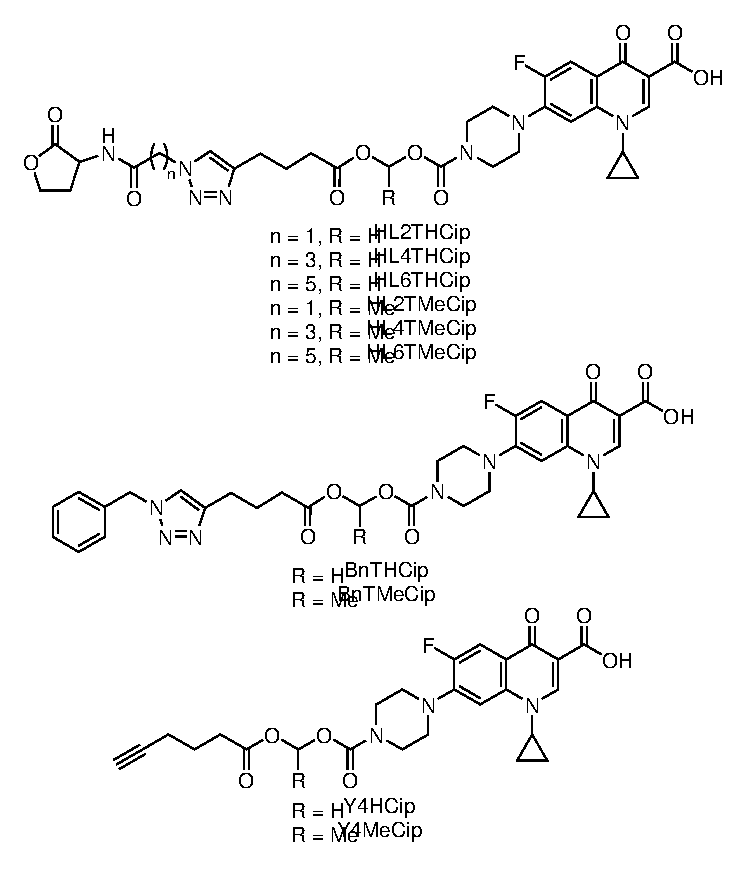
\includegraphics[scale=1]{finals_cleavable}
		\caption{The cleavable HSL-Cip conjugates.
 		\label{fgr:finals_cleavable}}
	\end{center}
\end{figure}

Here there was more success, although the activity was still not as high as for ciprofloxacin \compound{cmpd:Cip}.
The HSL-Cip conjugates with \textit{N}-(acetoxymethoxycarbonyl) linkers (R = H) showed activity at high concentrations. A longer linker seems to give higher activity; \compound{cmpd:HL4THCip} and \compound{cmpd:HL6THCip} showed activity comparable with ciprofloxacin \compound{cmpd:Cip} at high concentrations.
Unfortunately the control \compound{cmpd:BnTHCip} and alkyne \compound{cmpd:Y4HCip} with \textit{N}-(acetoxymethoxycarbonyl) linkers (R = H) showed higher activity than the conjugates, indicating that the HSL head wasn't contributing to the activity of the conjugates.

The conjugates with an \textit{N}-(acetoxyethoxycarbonyl) linker (R = Me) did not show any activity. This suggests that they either didn't enter cells or weren't suitable substrates for esterases.
The \textit{N}-(acetoxyethoxycarbonyl) linked alkyne (R = Me) did show some activity, indicating that maybe it could penetrate cells more easily than the conjugates due to its lower molecular weight and/or lower polarity.

\begin{figure}[H]
	\begin{center}
		\includegraphics[width=0.9\textwidth,trim={1cm 1cm 1cm 1cm},clip]{"Biochem - YM64_5h_C"}
		\caption{YM64 OD readings at 5 h for the cleavable HSL-Cip conjugates.\label{fgr:YM64_5h_cleavable}}
	\end{center}
\end{figure}
